\subsection{Function Shape}

\begin{figure}
	\centering
	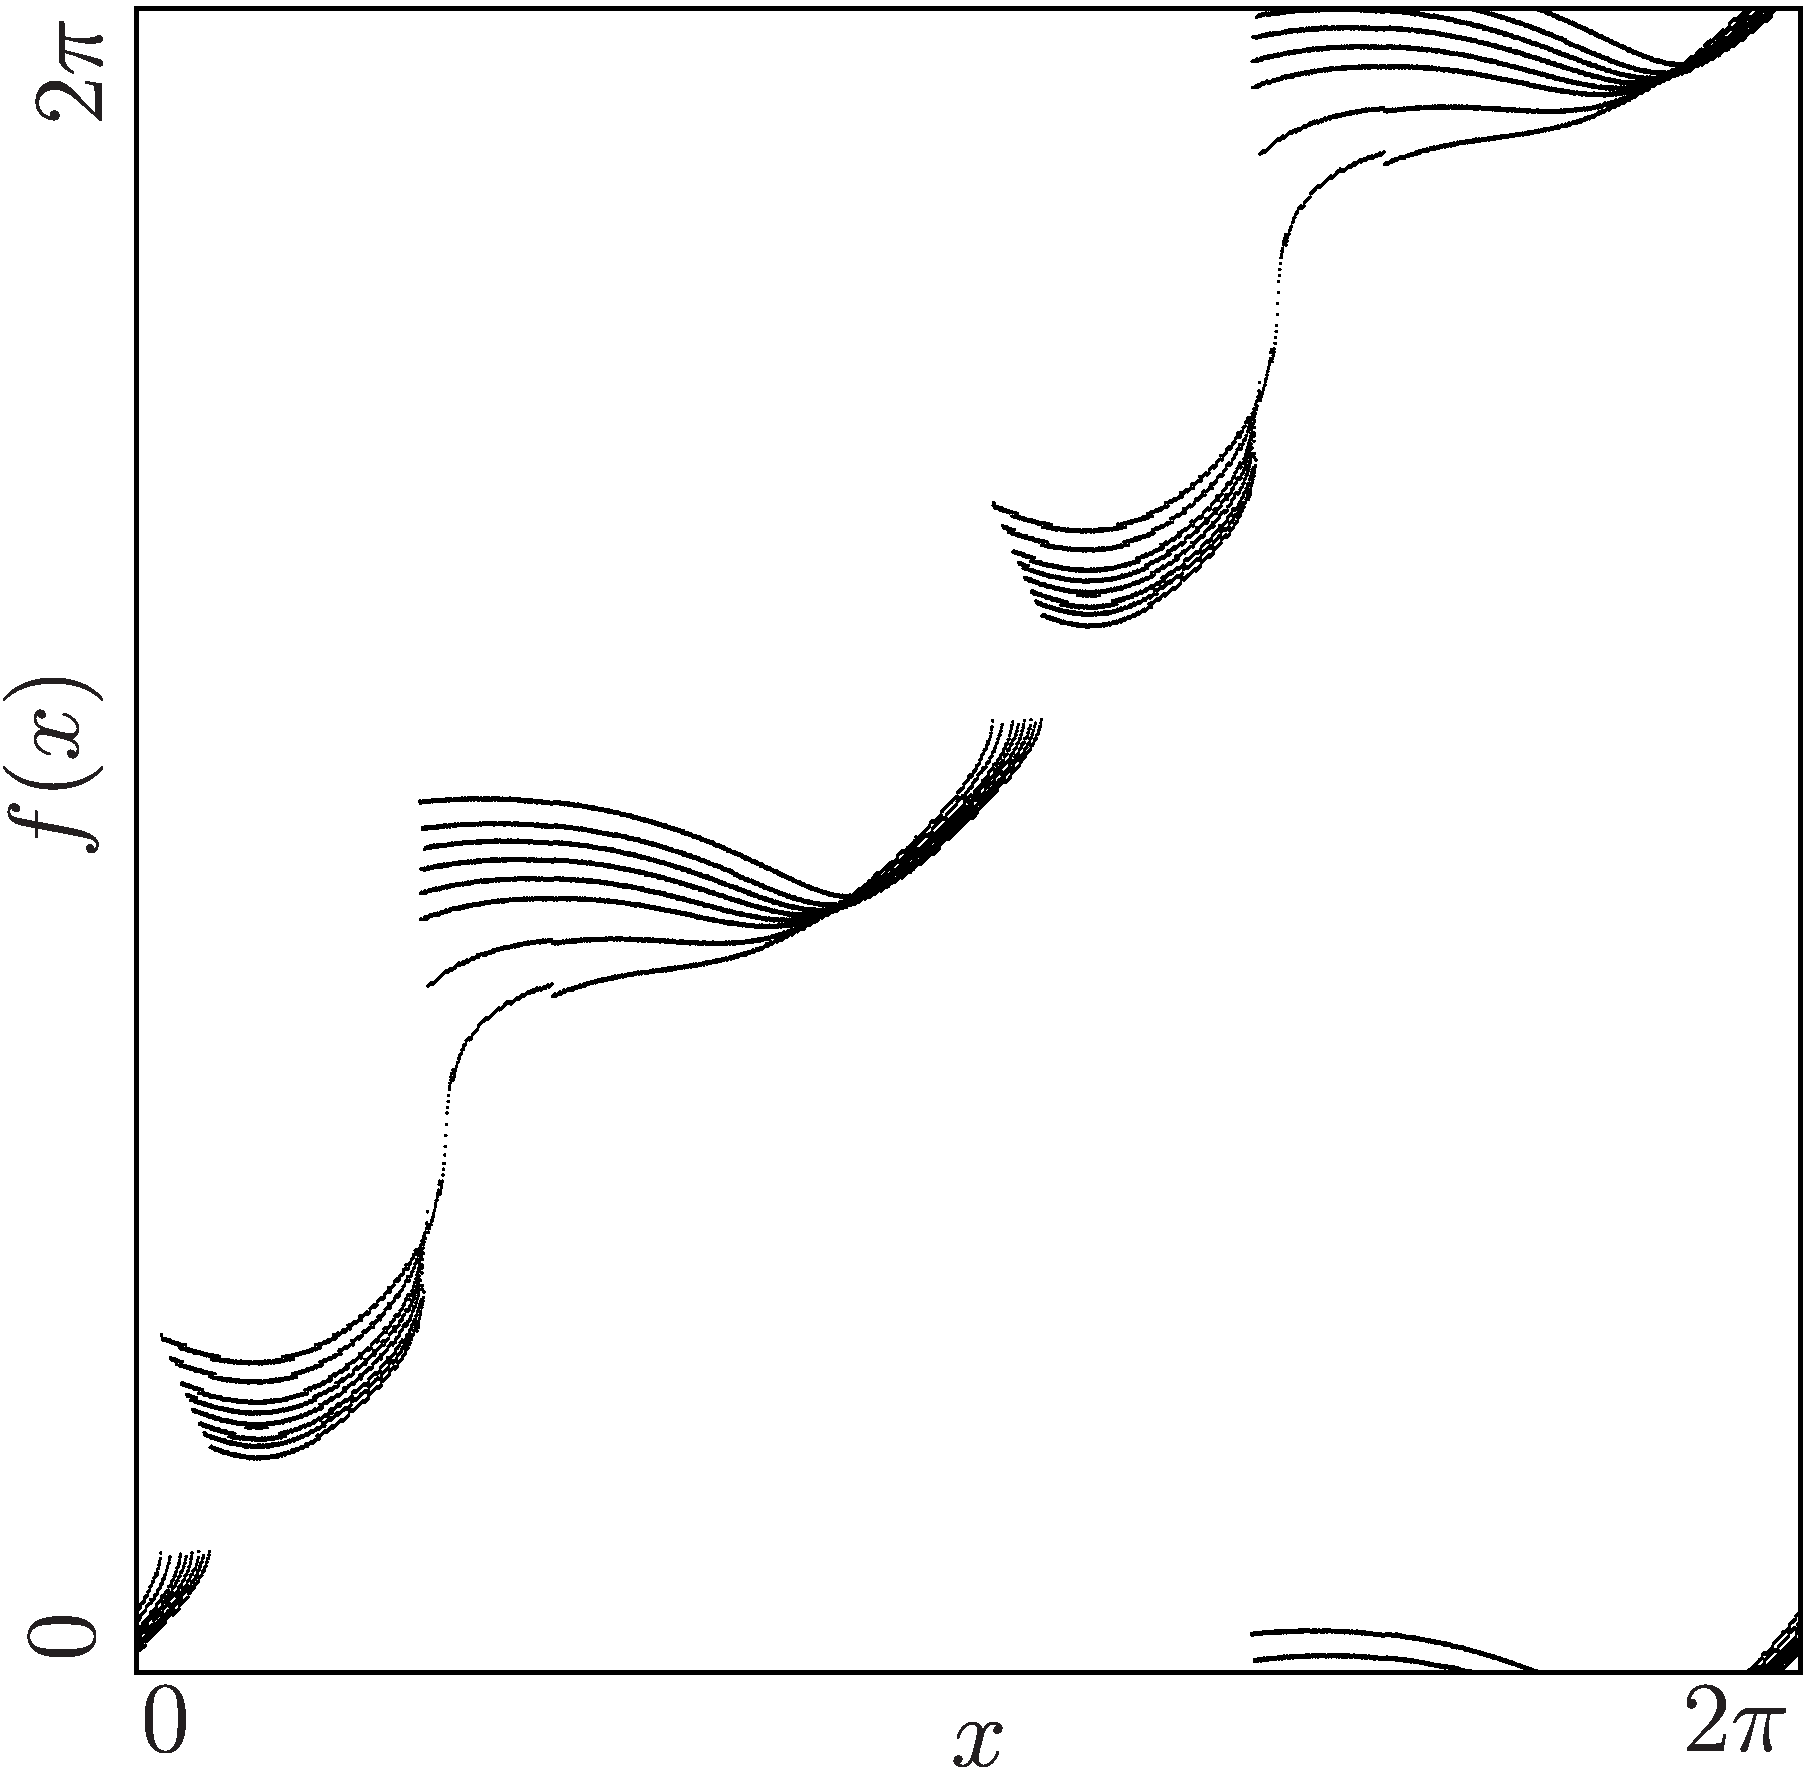
\includegraphics[width=.4 \textwidth]{99_Yunus/ParameterEffects/no/illustration.png}
	\caption[Shape of the original model function]{
		The shape of the original model function at the parameter values $E_0 = 15$ and $\chi_0 = 0.2$.
	}
	\label{fig:setup.char.shape}
\end{figure}

In this section, we examine the overall shape of the original model function.

\Cref{fig:setup.char.shape} shows the shape of the original model function.
We can see directly, that the function has 4 branches.
This is also evident from the model definition given in \Cref{sec:state.og.def}.
Also, we know from \Cref{sec:state.og.dynamics} that the model has symmetry, so the branches $f_\A$ and $f_\C$ are identical.
So are the branches $f_\B$ and $f_\D$.

There seem to be no fixed points in the parameter regions, we are interested in.
That means, the function is always larger than the bisector $y=x$.
Also, for the most part the derivative of the function is not extreme.
Meaning, it stays in the interval $(-1, 1)$ for the most part.
This property is also called contractive, since fixed points and cycles involving only points on contractive sections of a function are always stable.
